\documentclass[review]{elsarticle}

\usepackage{amsmath}
\usepackage{amssymb}
\usepackage{lineno,hyperref}
\usepackage{subcaption} 
\usepackage{booktabs}

\graphicspath{{./figures/}}
\modulolinenumbers[5]

\journal{XXX}

%%%%%%%%%%%%%%%%%%%%%%%
%% Elsevier bibliography styles
%%%%%%%%%%%%%%%%%%%%%%%
%% To change the style, put a % in front of the second line of the current style and
%% remove the % from the second line of the style you would like to use.
%%%%%%%%%%%%%%%%%%%%%%%

%% Numbered
%\bibliographystyle{model1-num-names}

%% Numbered without titles
%\bibliographystyle{model1a-num-names}

%% Harvard
%\bibliographystyle{model2-names.bst}\biboptions{authoryear}

%% Vancouver numbered
%\usepackage{numcompress}\bibliographystyle{model3-num-names}

%% Vancouver name/year
%\usepackage{numcompress}\bibliographystyle{model4-names}\biboptions{authoryear}

%% APA style
%\bibliographystyle{model5-names}\biboptions{authoryear}

%% AMA style
%\usepackage{numcompress}\bibliographystyle{model6-num-names}

%% `Elsevier LaTeX' style
\bibliographystyle{elsarticle-num}
%%%%%%%%%%%%%%%%%%%%%%%

\begin{document}

\begin{frontmatter}

\title{Radiation Damage from Neutron Scattering }
%\title{Radiation Damage\tnoteref{mytitlenote}}
%\tnotetext[mytitlenote]{INL Internship Summer 2017}

%% Group authors per affiliation:
\author{Sebastian Schunert, Marina Sessim, Daniel Schwen}
\address{Fuels Modeling and Simulation Department, Idaho National Laboratory, P.O Box 1625, Idaho Falls, ID 83415}
%\fntext[myfootnote]{Since 1880.}

%% or include affiliations in footnotes:
%\author[mymainaddress,mysecondaryaddress]{Elsevier Inc}
%\ead[url]{www.elsevier.com}

%\author[mysecondaryaddress]{Global Customer Service\corref{mycorrespondingauthor}}
%\cortext[mycorrespondingauthor]{Corresponding author}
%\ead{support@elsevier.com}

%\address[mymainaddress]{1600 John F Kennedy Boulevard, Philadelphia}
%\address[mysecondaryaddress]{360 Park Avenue South, New York}

\begin{abstract}

\end{abstract}

\begin{keyword}
Radiation damage\sep Elastic scattering \sep Inelastic scattering
%\MSC[2010] 00-01\sep  99-00
\end{keyword}

\end{frontmatter}

\linenumbers

\section{Introduction}

The purpose of this report is to derive expressions for the elastic and inelastic neutron recoil cross sections dependent only on quantities that can be obtained easily from fundamental data such as the National Nuclear Data Center~\cite{NNDC}. Recoil cross sections are essential to compute isotope, angle and energy dependent recoil rates given detailed neutron distribution in phase space that can be computed by a radiation transport code. In particular, the recoil cross sections are used in the Rattlesnake radiation transport code~\cite{RattlesnakeTheoryManual} to compute recoil rate distributions that are passed on to the Magpie [Ref?] glue application for computing primary knock-on atom (PKA) distribution rates in turn used for coupled binary-collision Monte-Carlo/FEM calculations. Elastic and inelastic neutron scattering events are important interactions initiating radiation damage cascades especially in structural materials.


%**********************************************************************************************************************************************************************************************%
\section{Scattering Kinematics}

Following Fig. \ref{fig:kinematic_sketch}, we denote the speed of the neutron by $v$ and the speed of the recoil atom as $V$. The subscript shall denote in which frame of reference the speed is measured, $v_l$ is measured in the laboratory (LAB) frame and $v_c$ is measured in the center of mass (CM) frame. Primed speeds, e.g. $v_c'$, denote states after the collision, while un-primed speeds denote states prior to the collision. 
The scattering angle in the CM frame is denoted by $\phi$, while the recoil angle in the LAB frame is denoted by $\alpha$. We denote the cosine of these angles as $\mu_l = \cos \alpha$ and $\mu_c = \cos \phi$.
Within the following development, some expressions hold for both elastic and inelastic scattering, while some hold only for one of them. We shall adopt the convention that unless otherwise stated, expressions hold for both elastic and inelastic scattering.


\begin{figure}
	\centering
	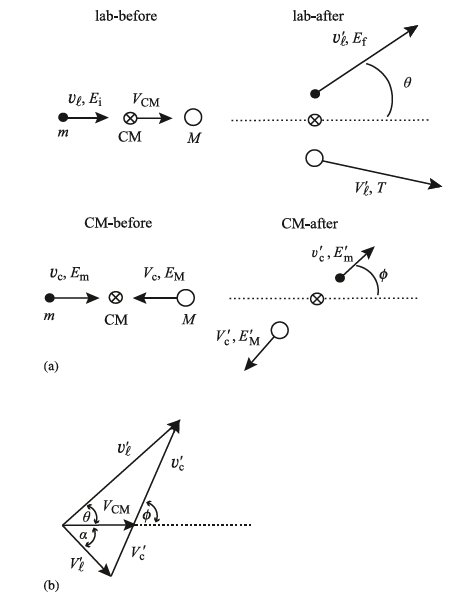
\includegraphics[width=0.8\linewidth]{triangles_GWas}
	\caption{Relationship between angles in CM and laboratory frame~\cite{GaryWas}.}
	\label{fig:kinematic_sketch}
\end{figure}

\subsection{Relationship between Recoil Angles in CM and LAB frames}\label{sec:dependence_mu_l_mu_c}
First, we point out that the mass of the of the neutron is set to unity $m=1$, while the mass of the recoil atom is its mass number $M=A$. The speed of the center of mass $v_{CM}$ is given by~\cite{Duderstadt1976}:

The velocity of the center of mass $v_{CM}$ is given by~\cite{Duderstadt1976}:
\begin{equation}
	v_{CM} = \frac{1}{m+M}(m v_l + M V_l) = \left( \frac{1}{1+A}\right) v_l
\end{equation}
The relationship between the velocities on the LAB and CM frame is given by:
\begin{equation}
	v_c = v_l - v_{CM} = \frac{A}{A+1}v_l 
\end{equation}
and
\begin{equation}\label{eq:V_c}
	V_c = - v_{CM} = \frac{1}{A+1}v_l
\end{equation}
where we have assumed that the target nucleus is at rest before the collision. 

\subsubsection{Elastic Scattering}
Following~\cite{GaryWas} we can formulate energy and momentum conservation in the CM frame:
\begin{align} \label{eq:elastic_energy_momentum_balance}
  v_c - V_c A  &= 0 \nonumber \\
  v_c' - V_c' A &= 0 \nonumber \\
  \frac{1}{2} v_c^2 + \frac{1}{2} A V_c^2 &= \frac{1}{2} v_c'^2 + \frac{1}{2} A V_c'^2.
\end{align}
From Eq.~\ref{eq:elastic_energy_momentum_balance} we can conclude:
\begin{align}\label{eq:rotated_vel}
  V_c &= V_c' \nonumber \\
  v_c &= v_c',
\end{align}
which is a well known result stated by~\cite{Duderstadt1976} as (paraphrasing): the magnitude of the CM velocities of the projectile and target are not changed but only rotated.
From Eq.~\ref{eq:rotated_vel} and Eq. \ref{eq:V_c} it follows that $|V_c' | = |v_{CM}|$. 

Focusing on the triangle spanned by $v_{CM}$, $V_l'$, and $V_c'$ in Fig.~\ref{fig:kinematic_sketch} (b), we realize that the triangle is isosceles because $|V_c' | = |v_{CM}|$. Hence, we have:
\begin{equation}
  \phi + 2 \alpha = \pi \rightarrow \alpha = \frac{1}{2} (\pi - \phi).
\end{equation}
Taking the cosine on both sides leads to:
\begin{equation}\label{eq:muL_mu_C_elastic}
 \mu_l = \cos  \left( \frac{\pi}{2} - \frac{\phi}{2} \right) =  \sin  \frac{\phi}{2} = \pm \sqrt{\frac{1 - \cos \phi }{2} } = \pm \sqrt{\frac{1 -\mu_c }{2} } .
\end{equation}
Finally, we need to specify which sign in Eq. \ref{eq:muL_mu_C_elastic} is correct. The recoil angle in the LAB frame $\alpha$ must be between $0$ and $\phi/2$, i.e. the recoil atom cannot be backscattered. Hence, $\mu_l > 0$ and we find that:
\begin{equation}\label{eq:muL_mu_C_elastic2}
 \mu_l =  \sqrt{\frac{1 -\mu_c }{2} } .
\end{equation}

\subsection{Inelastic Scattering}
The relationship between CM and LAB angles is more complicated for inelastic scattering because the triangle spanned by $v_{CM}$, $V_l'$, and $V_c'$ in Fig.~\ref{fig:kinematic_sketch} (b) is \textit{not}
isosceles. From the same triangle, we infer by simple geometric considerations along the x and y directions:
\begin{align}\label{eq:mu_l_mu_c_inelastic1}
  \sin \alpha ~V_l' &= \sin \phi ~V_c' \nonumber\\
 \cos \alpha ~V_l'  &= v_{CM} - \cos \phi ~V_c'.
 \end{align} 
Taking the ratio of the first and second Eq.~\ref{eq:mu_l_mu_c_inelastic1} gives:
\begin{equation}\label{eq:mu_l_mu_c_inelastic2}
  \tan \alpha = \frac{\sin \phi }{\frac{V_c}{V_c'} - \cos \phi} .
 \end{equation}
It now remains to determine the ratio $V_c / V_c'$. To this end, the energy and momentum balance Eq.~\ref{eq:elastic_energy_momentum_balance} is extended to inelastic scattering by introducing the
Q-value of the reaction $Q_j$, where $j$ indicates the excitation level a particular inelastic scattering event triggers:
\begin{align} \label{eq:inelastic_energy_momentum_balance}
  v_c - V_c A  &= 0 \nonumber \\
  v_c' - V_c' A &= 0 \nonumber \\
 Q_j +  \frac{1}{2} v_c^2 + \frac{1}{2} A V_c^2 &= \frac{1}{2} v_c'^2 + \frac{1}{2} A V_c'^2,
\end{align}
where $Q_j < 0$.
From~\ref{eq:inelastic_energy_momentum_balance} we derive the following relationship between $V_c$ and $V_c'$:
\begin{equation}\label{eq:V_c_inelastic_pre}
  V_c'^2 = V_c^2 + \frac{2 Q_j}{A(A+1)} \rightarrow \left( \frac{V_c'}{V_c} \right)^2 = 1 + \frac{2 Q_j}{A(A+1) V_c^2}.
\end{equation}
The square oif the initial velocity $V_c^2$ can can be replaced by the $v_l$ using Eq.~\ref{eq:V_c}:
\begin{equation}
  V_c^2 = \frac{2}{(A+1)^2} \frac{1}{2} v_l^2 =  \frac{2E}{(A+1)^2},
\end{equation}
where $E$ is the initial energy of the neutron in the LAB frame. Finally we obtain:
\begin{equation}\label{eq:V_c_inelastic}
   \left( \frac{V_c}{V_c'} \right) = \left(1 + \frac{ Q_j}{E}  \frac{A+1}{A} \right)^{-1/2}.
\end{equation}
Introducing the threshold energy $E_t$ and the dimensionless neutron energy $\Delta$ by:
\begin{align}
  E_t & = \frac{(A+1)}{A}\left |Q_j\right |  \nonumber \\
  \Delta &= \frac{E_t}{E},
\end{align}
we can simplify Eq. \ref{eq:V_c_inelastic} to:
\begin{equation}\label{eq:V_c_inelastic2}
   \left( \frac{V_c}{V_c'} \right) = \left(1 - \Delta \right)^{-1/2}.
\end{equation}
Using Eq.~\ref{eq:V_c_inelastic2} in Eq.~\ref{eq:mu_l_mu_c_inelastic2} gives:
\begin{equation}\label{eq:tan_alpha_inelastic}
   \tan \alpha =  \frac{\sin \phi }{ \left(1 - \Delta \right)^{-1/2}  - \cos \phi}.
\end{equation}
We now want to write the right hand side of Eq~\ref{eq:tan_alpha_inelastic} in terms of $\mu_c$. First, we note that
$\sin \phi \ge 0$ because $0 \le \phi \le \pi$. Hence, we can replace $\sin \phi$ with $\sqrt{1 - \mu_c^2}$ as opposed to using the opposite sign.
For convenience we denote the right hand side of Eq~\ref{eq:tan_alpha_inelastic} as $f(\mu_c)$:
\begin{equation}
f(\mu_c) =  \frac{\sqrt{1 - \mu_c^2}}{ \left(1 - \Delta \right)^{-1/2}  - \mu_c},
\end{equation}
Note that since $0 < \Delta \le 0$, $\left(1 - \Delta \right)^{-1/2} \ge 1$ and consequently $f(\mu_c) > 0$.
%Note that $\mu_c < \mu_{c,t}$ with $\mu_{c,t}$ being the threshold angle. We will determine the threshold angle in section XX. 
Writing Eq.~\ref{eq:tan_alpha_inelastic} in terms of $\mu_l$ gives:
\begin{equation}\label{eq:mu_l_mu_c_inelastic_final}
  \mu_l = \sqrt{ \frac{1}{1 + f^2 (\mu_c)} },
\end{equation}
where we immediately asserted $\mu_l >0$ when taking the square root. 

\section{Energy Transfer to the Recoil Nucleus - Elastic Scattering}
In this section, we derive the relationship between the energy of the neutron prior to the collision $E$, the energy of the recoil nucleus after the collision $T$, and the
scattering cosine in the CM frame $\mu_c$. If two of the three quantities are given, the third is determined and can no longer be chosen at will.
It is convenient to define the mass fraction $\gamma$~\cite{GaryWas}:
\begin{equation}
	\gamma = \frac{4 A}{(A+1)^2}
\end{equation}
[Note this mass fraction is universally applicable to elastic and inelastic scattering even though it is contained in the elastic scattering energ transfer section.]
For elastic scattering, the relationship between $E$, $T$ and $\mu_c$ is given by~\cite{GaryWas}:
\begin{equation}\label{eq:T_elastic}
	T = \frac{\gamma}{2} E (1-\mu_c).
\end{equation}
Solving for $\mu_c$ gives:
\begin{equation}
	\mu_c = 1 - \frac{2 T}{\gamma E}
	\label{eq:muc}
\end{equation}

\section{Energy Transfer to the Recoil Nucleus - Inelastic Scattering}
The following expression is adopted from~\cite{GaryWas}:
\begin{equation}\label{eq:T_inelastic_pre}
  T = \frac{\gamma}{2} E - \frac{\gamma}{2} \left[ E \left( E + Q_j \frac{A+1}{A} \right)  \right]^{1/2} \mu_c + \frac{Q_j}{A+1},
\end{equation}
where it is again stressed that $Q_j < 0$. We can rewrite this equation in a more convenient form by using the dimensionless neutron energy $\Delta$:
\begin{equation}\label{eq:T_inelastic}
  T = \frac{\gamma}{2} E \left (  1 - \mu_c \sqrt{1 - \Delta} - \frac{1}{2} \Delta \right ).
\end{equation}


\section{Limits on the Scattering Angles and Energy Transfer}

\subsection{Scattering Angle in CM}
It is obvious from Fig.~\ref{fig:kinematic_sketch} (b) that the scattering angle in the CM frame $\phi$ satisfies:
\begin{equation}
   0 \le \phi \le \pi.
\end{equation}
An angle $\phi > \pi$ would simply reflect Fig.~\ref{fig:kinematic_sketch} (b) about the x-axis. It follows that
\begin{equation}
   -1 \le \mu_c \le 1.
\end{equation}

\subsection{Recoil Angle in LAB}
The recoil angle in the  LAB frame must be between $0$ and $\pi/2$:
\begin{equation}
   0 \le \alpha \le \pi /2.
\end{equation}
This can most easily be seen when considering the triangle $V_l'$, $v_{CM}$, $V_c'$ in Fig.~\ref{fig:kinematic_sketch} (b). For both elastic and inelastic scattering we see from Eq. \ref{eq:V_c_inelastic} that
$V_c' \le V_c = v_{CM}$. Hence, regardless of the CM scattering angle $\phi$ with $0 \le \phi \le \pi$ the vertex opposite of $v_{CM}$ can never be located to the left of the vertex opposite $V_c'$ proving the 
limits stated above.  

\subsection{Recoil Energy for Elastic Scattering}
The case $\phi=0$ ($\mu_c=1$) corresponds to a grazing collision where the neutron loses no energy and recoil nucleus remains at rest; while $\phi=\pi$ ($\mu_c=-1$) corresponds to a head on collision,
where the neutron loses the maximum amount of energy and the recoil receives the maximum amount of energy. Using Eq.~\ref{eq:T_elastic} with $\mu_c=1$ and $\mu_c=-1$ gives:
\begin{equation}
    0 \le T \le \gamma E.
\end{equation}

\subsection{Threshold Neutron Energy, and Recoil Energy for Inelastic Scattering}
Neutrons with $\Delta > 1$ cannot cause inelastic scattering reactions. This is consistent with square root terms of the form $\sqrt{1 - \Delta}$ which would become imaginary if $\Delta > 1$. However, a more stringent requirement is that the CM scattering cosine is within physical bounds $-1 \le \mu \le 1$. For $E \rightarrow E_t$ from above, $\mu_c$ is strictly monotonically decreasing. Given an arbitrary value of the recoil energy $T$, $\mu_c=-1$ is usually not assumed for $E = E_t$. The minimum possible neutron energy for a given recoil energy is:
\begin{equation}\label{eq:E_min}
   E_{min}(T) = \frac{\left(T (A+1) + \left |Q_j \right|  \right)^2}{4 A T}. 
\end{equation}
Further analysis shows that $E_{min}$ assumes a minimum at:
\begin{equation}
   T = \frac{\left| Q_j \right|}{A+1},
\end{equation}
where we have
\begin{equation}
  E_{min}(\frac{\left| Q_j \right|}{A+1}) = E_t.
\end{equation}

The maximum and minimum energy of the recoil are denoted by $T_{min}(E)$ and $T_{max}(E)$ and they occur for $\mu_{c} = 1$ and $\mu_c=-1$, respectively. 
For convenience we define:
\begin{equation}
   g(\mu_c, \Delta) = \frac{\gamma}{2} E \left( 1 -\mu_c  \sqrt{1 - \Delta} - \frac{1}{2} \Delta  \right).
\end{equation}
The function $g(\mu_c, \Delta)$ is plotted for $\mu_c=1$ and $\mu_c=-1$ in Fig.~\ref{fig:g_mu_delta}.
The maximum and minimum recoil energy given a neutron energy are given by:
\begin{align}\label{eq:T_min_max}
  T_{min}(E) &=  \frac{\gamma}{2} E \left (  1 - \sqrt{1 - \Delta} - \frac{1}{2} \Delta \right ) \nonumber \\
  T_{max}(E) &=  \frac{\gamma}{2} E \left (  1 + \sqrt{1 - \Delta} - \frac{1}{2} \Delta \right ).
\end{align}
It should be noted that $T_{min}$ and $T_{max}$ are monotonically decreasing and increasing with neutron energy $E$, respectively. 

\begin{figure}
	\centering
	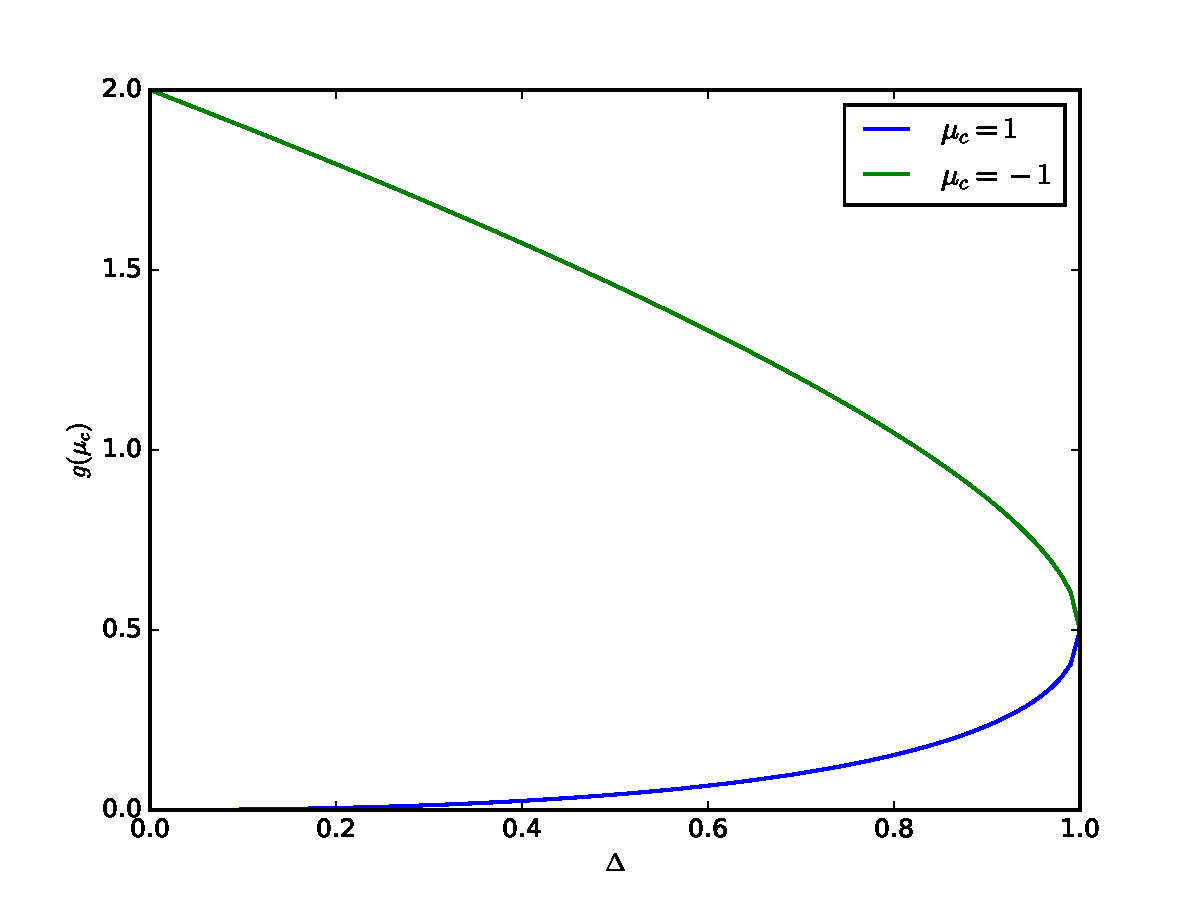
\includegraphics[width=0.75\linewidth]{g_mu_delta.pdf}
	\caption{Function $g(\mu_c, \Delta)$ plotted vs. $\Delta$ for $\mu_c=1$ (minimum recoil) and $\mu_c=-1$ (maximum recoil).}
	\label{fig:g_mu_delta}
\end{figure}

\subsection{Limits of Inleastic Scattering Energies considering Neutron and Recoil Energy Bins}
In this section we consider the case, where neutron and recoil energy limits are desired for a transfer of neutrons with energies $E_l \le E \le E_u$ causing recoils with energies $T_l \le T \le T_u$. The final energy limits shall be denoted by $E_{\downarrow}$, $E_{\uparrow}$, $T_{\downarrow}$, and $T_{\uparrow}$ for the lower and upper energy limits of the neutron and recoil, respectively. These limits denote possible scattering interactions consistent with the energy group boundaries. To illustrate the recoil energy limits, we consider Fig.~\ref{fig:energy_boundaries}. The curves representing $T_{min}(E)$ and $T_{max}(E)$ are depicted in green and blue, respectively. They share a common point at $E=E_t$, $T=\frac{|Q_j|}{A+1}$ with a common vertical tangent $E=E_t$ depicted in red. The energy group boundaries $E_l$, $E_u$, $T_l$ and $T_u$ are depicted in orange. 

The limits on the neutron energy are:
\begin{align}
 E_{\downarrow} & = \left\{ \begin{array}{ll}
         E_l, & E_l > E_t \\
         E_t, & E_l \le E_t  \\
         \end{array}
         \right .     \nonumber \\
E_{\uparrow} & = \left\{ \begin{array}{ll}
         E_u, & E_l > E_t \\
         \text{neutrons cannot scatter}, & E_u \le E_t  \\
         \end{array}
         \right .      .   
\end{align} 
In Fig.~\ref{fig:energy_boundaries} $E_t< E_l < E_u$ and hence $E_{\downarrow}=E_l$ and $E_{\uparrow} = E_u$. 
The range of possible recoil energies is given by the overlap of two areas: first, the range $[T_l, T_u]$ and second the physically possible minimum and maximum recoil energies $[T_{min}, T_{max}]$. The upper limit is given by:
\begin{equation}
   T_{\uparrow} = \min \left( T_{max}(E_{\uparrow}), T_u \right).
\end{equation}
Note that the largest value of $T_{max}$ is assumed for the largest $E$. The lower limit is given by:
\begin{equation}
   T_{\downarrow} = \max \left( T_{min}(E_{\uparrow}), T_l \right).
\end{equation}
Again it should be noted that the minimum of $T_{min}$ is assumed for the largest neutron energy. 
In Fig.~\ref{fig:energy_boundaries} the region of permissible scattering is marked by the green box.
It should be noted that the fraction of the scattering processes located in the green box but above the blue $T_{max}$ line are impossible which must be taken into consideration when a particular $E \rightarrow T$ set is considered.
Finally, the scattering process is impossible if:
\begin{align}
   E_u & < E_t \nonumber \\
   T_{\uparrow} & < T_l \nonumber \\
   T_{\downarrow} & > T_u. 
\end{align}

\begin{figure}
	\centering
	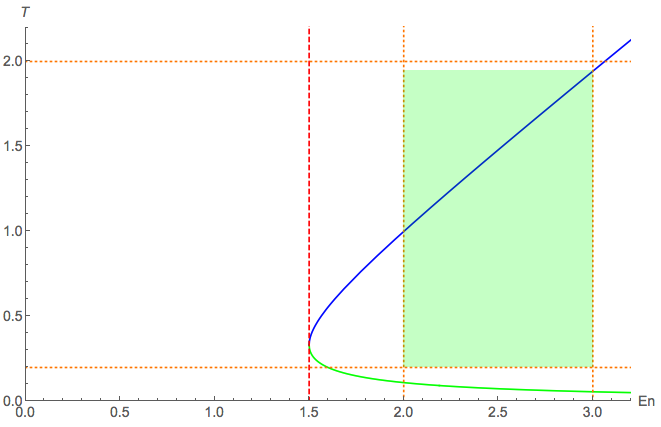
\includegraphics[width=1.0\linewidth]{energy_boundaries.png}
	\caption{Diagram in $E$-$T$ space to illustrate limits on recoil energy.}
	\label{fig:energy_boundaries}
\end{figure}

    
%**********************************************************************************************************************************************************************************************%
\section{Role of De-excitation Gamma Rays}
The de-excitation gamma ray is released by the nucleus after the inelastic scattering event concludes. The process of inelastic scattering, considered from before the interaction to after the gamma is released, is a three-body problem. However, as the gamma ray is released after the neutron capture, compound nucleus formation, and neutron release it can be broken up into two two-body problems. The kinematics of the first two-body problem are discussed above, while the second two-body problem is discussed in this section. The central question is whether the momentum of the de-excitation gamma is large compared to the overall momentum in the system. 

The absolute value of momentum of the gamma ray is:
\begin{equation}\label{eq:momentum_gamma_ray}
  |p_{\gamma} |= \frac{|Q_j|}{c},
\end{equation}
where $c$ is the speed of light. The momentum of the neutron prior to collision is:
\begin{equation}
  |p_n| = \sqrt{2 E m_n},
\end{equation}
where $m_n$ is the mass of the neutron. Since $E > \frac{|Q_j| (A+1)}{A} > |Q_j|$, we conclude:
\begin{equation}
  |p_n| > \sqrt{2 |Q_j| m_n}.
\end{equation}
For the ratio $r = |p_n| / |p_{\gamma}|$ it follows that:
\begin{equation}
  r > c \sqrt{\frac{2 m_n}{|Q_j|}}.
\end{equation}
Substituting $c\approx 3 \times 10^8 $ m/s and $m_n\approx 1.7 \times 10^{-27}$ kg and rounding generously we obtain:
\begin{equation}
 r   \gtrapprox 42,000 \sqrt{\frac{1}{|Q_j| \text{(eV)}}}
\end{equation}
Typical values for $E_t$, $|Q_j|$, and the lower limit of $r$ are compiled in Table~\ref{table:typical_Q}. It is obvious that even for the highest threshold energies the momentum in the neutron are
much larger than the momentum imparted into the de-excitation gamma ray. 
As a rule of thumb, the Q-value for inelastic scattering reactions is higher for light nuclides. As light nuclides receive high recoils from elastic scattering reactions and at the same time allow only a fraction of the neutrons to interact with them in the inelastic scattering mode, inelastic scattering is relatively unimportant for light nuclei. Conversely, heavy nuclides do not allow energy transfer by elastic scattering, but
have low threshold energies making inelastic scattering important. However, for heavy nuclei the momentum of the gamma ray is even smaller than in the case of light nuclei. In conclusion, the momentum of the gamma ray is small for all cases compared with the overall momentum in the system, but it tends to be smallest for cases where inelastic scattering matters most. Hence, for the purpose of simulating inelastic scattering reactions, the secondary de-excitation can be ignored when determining the direction of the recoil nucleus.

\begin{table}[htbp]
\caption{Threshold energies, Q-values, and neutron to gamma momentum ratios for several nuclides.}
\centering
\begin{tabular}{c c c c}
\toprule
Nuclide & $E_t$ (MeV) & $|Q_j|$ (MeV) & $r_{min}$ \\
\midrule
$^{12}$C & 4.4 & 4.15 & 20 \\
$^{16}$0 & 6.1 & 5.74 & 17.5 \\
$^{23}$Na & 0.45 & 0.43 & 64 \\
$^{238}$U & 0.045 & 0.045 & 198 \\
\bottomrule
\end{tabular}
\label{table:typical_Q}
\end{table}


%**********************************************************************************************************************************************************************************************%
\section{Recoil Production Rate}
The number of recoils of nuclide type $n$, with recoil energies in $dT$ about $T$, and directions within $d \hat{\Omega}_T$ about $\hat{\Omega}_T$ is denoted by $R_n(T,\hat{\Omega}_T)$. 
It can be computed by:
\begin{equation}
	R_n(T,\hat{\Omega}_T) = N_n  \int\limits_{4\pi} d \hat{\Omega} \int\limits_0^\infty dE  \sigma_{r,n}(E \rightarrow T, \hat{\Omega} \rightarrow \hat{\Omega}_T) \psi(E, \hat{\Omega}),
\label{eq:rate}
\end{equation}
where $N_n$ is the number density of nuclide $n$, $E$ is the incident neutron energy, T is the energy transferred to the recoil atom, $\hat{\Omega}$ is the incident neutron direction, $\hat{\Omega}_T$ is the scattered neutron direction, $\psi$ is the angular neutron flux, and $\sigma_{r,n}(E \rightarrow T, \hat{\Omega} \rightarrow \hat{\Omega}_T)$ is the microscopic, double differential recoil cross section for nuclide $n$. It will be the overarching task of this section to derive a viable expression for $R_n(T,\hat{\Omega}_T)$ in terms of fundamental properties.

In the vast majority of materials, the recoil cross section only depends on the cosine of the angle between incident neutron direction and recoil direction, i.e. $\mu_l =\hat{\Omega} \cdot \hat{\Omega}_T$~\cite{lewis1984}. Consequently, we can rewrite the cross section as: $\sigma_{r,n}(E \rightarrow T, \mu_l)$.

Consistent with the multigroup formalism for treating energy dependence of neutron populations, the energy range of the recoils are broken up into groups indexed by $j=1,...,J$; consistent with treatment of neutrons the energy groups are numbered in order of descending energy, i.e. the highest energy group has index j, while the lowest energy group has index $J$. The $j$-th group comprises the energy range $T_{j+1} \le T < T_j$. Similarly, neutron energy groups are introduced indexed by $g=1,...,G$ following the same convention. Integrating Eq.~\ref{eq:rate} over the energy range of recoil group $j$ leads:
\begin{equation}
  R_{n,j}(\hat{\Omega}_T) =  N_n  \int\limits_{4\pi} d \hat{\Omega} \int\limits_{T_{j+1}}^{T_j} dT \int\limits_0^\infty dE  \sigma_{r,n}(E \rightarrow T, \mu_l) \psi(E, \hat{\Omega}).
\end{equation} 
The integral over all neutron energies is broken up into contributions from each neutron energy group:
\begin{equation}\label{eq:mg_R_1}
  R_{n,j}(\hat{\Omega}_T) =  N_n  \sum\limits_{g=1}^G \int\limits_{4\pi} d \hat{\Omega} \int\limits_{T_{j+1}}^{T_j} dT \int\limits_{E_{g+1}}^{E_g} dE  \sigma_{r,n}(E \rightarrow T, \mu_l) \psi(E, \hat{\Omega}).
\end{equation} 
In the neutron multigroup framework, only the group fluxes $\psi_g(\hat{\Omega})$ are available:
\begin{equation}
  \psi_g(\hat{\Omega}) =  \int\limits_{E_{g+1}}^{E_g} dE \psi(E,\hat{\Omega}).
\end{equation} 
The recoil rate can formally be written in terms of $\psi_g$:
 \begin{align}\label{eq:mg_R_2}
  R_{n,j}(\hat{\Omega}_T) &=  N_n  \sum\limits_{g=1}^G \int\limits_{4\pi} d \hat{\Omega} \sigma_{r,n}^{g \rightarrow j} (\mu_l) \psi_g(\hat{\Omega}) \nonumber \\
  \sigma_{r,n}^{g \rightarrow j} (\mu_l)& = \frac{\int\limits_{T_{j+1}}^{T_j} dT \int\limits_{E_{g+1}}^{E_g} dE  \sigma_{r,n}(E \rightarrow T, \mu_l) \psi(E, \hat{\Omega})}{\psi_g(\hat{\Omega})}.
\end{align} 
during the preparation of the cross sections, the spectrum, i.e. $\psi(E,\hat{\Omega})$, is unknown and hence we need to guess a spectrum that we denote by $\xi(E)$. Using the approximated spectrum, we
can approximate $ \sigma_{r,n}^{g \rightarrow j} (\mu_l)$:
\begin{align}\label{eq:sigma_definition_1}
    \sigma_{r,n}^{g \rightarrow j} (\mu_l)& \approx \frac{1}{\xi_g}\int\limits_{T_{j+1}}^{T_j} dT \int\limits_{E_{g+1}}^{E_g} dE  \sigma_{r,n}(E \rightarrow T, \mu_l) \xi(E) \nonumber \\
     \xi_g &= \int\limits_{E_{g+1}}^{E_g} dE \xi(E).
\end{align}

It is convenient to represent the dependence of  $\sigma_{r,n}^{g \rightarrow j}$ on $\mu_l$ as a series expansion in Legendre polynomials truncated at a sufficently high order $L$:
\begin{equation}\label{eq:leg_expansion_sigma}
   \sigma_{r,n}^{g \rightarrow j} (\mu_l) = \sum\limits_{k=0}^{L} \frac{(2k +1)}{\Delta \mu_l} \sigma_{r,n,l}^{g \rightarrow j} P_k^*(\mu_l) H(\mu_l, \mu_{l,min}, \mu_{l,max}),
\end{equation}
where $\mu_{l,min}$ and $\mu_{l,max}$ are minimum and maximum LAB scattering cosines for energy group combination $g$ to $j$ (note, these are \textit{not} $0$ and $1$ corresponding to $\alpha=\pi/2$ and $\alpha=0$ respectively), $\Delta \mu_l = \mu_{l,max} - \mu_{l,min}$, $P_l^*(\mu_l)=P_l \left(  2 \frac{\mu_l - \mu_{l,min}}{\Delta \mu_l} - 1  \right)$ with $P_k$ being standard Legendre polyonomials of order $k$ of which the first few are $1, \mu_l, 1/2(3 \mu_l^2 - 1), ...$, and finally $H(\mu_l, \mu_{l,min}, \mu_{l,max})$ is given by:
\begin{equation}
  H(\mu_l, \mu_{l,min}, \mu_{l,max}) = \left\{ \begin{array}{ll}
         1 & \mu_{l,min} \le  \mu_l \le  \mu_{l,max};\\
         0 & \text{else}.\end{array} \right.
\end{equation}
The Legendre polynomials satisfy the following orthogonality property:
\begin{equation}
	\int\limits_{\mu_{l,min}}^{\mu_{l,max}} d \mu_l P^*_k(\mu_l) P^*_{i}(\mu_l) = \frac{\Delta \mu_l}{2k +1} \delta_{k,i},
\end{equation}
where $\delta_{k,i}$ is the Kronecker delta.
The minimum and maximum scattering cosines in the LAB frame can be determined from the smallest and largest $T / E$ ratio for pairing $g$ and $j$ as follows:
\begin{align}\label{eq:min_max_mu}
   \left( \frac{T}{E} \right)_{min} = \left( \frac{T_{j+1}}{E_{g}}   \right) \rightarrow \mu_{c,max} \rightarrow \mu_{l,min} \nonumber \\
    \left( \frac{T}{E} \right)_{max} = \left( \frac{T_{j}}{E_{g+1}}   \right) \rightarrow \mu_{c,min} \rightarrow \mu_{l,max},
\end{align}
where Eqs.~\ref{eq:muc} and~\ref{eq:muL_mu_C_elastic2} are used for elastic scattering and Eqs.~\ref{eq:T_inelastic} and~\ref{eq:mu_l_mu_c_inelastic_final} are used for inelastic scattering.
(this is obvious for elastic, but verify this for inelastic as well).

Multiplying Eq.~\ref{eq:leg_expansion_sigma} with $P_i^*$ and integrating over $\mu_l$ within $\mu_{l,min}$ and $\mu_{l,max}$ gives:
\begin{equation}\label{eq:sigma_coefficient}
   \sigma_{r,n,l}^{g \rightarrow j} = \int\limits_{\mu_{l,min}}^{\mu_{l,max}} d\mu_l P^*_i(\mu_l)\sigma_{r,n}^{g \rightarrow j} (\mu_l) .
\end{equation}
Before continuing, the dependence of the recoil cross section on $T$, $E$ and $\mu_l$ is discussed. In section~\ref{sec:dependence_mu_l_mu_c} we determined a relationship of the scattering cosine in the LAB and CM frame, where for elastic scattering $\mu_l$ is a function of $\mu_c$ only, while for inelastic scattering $\mu_l$ also depends on $E$. As pointed out previously $T$, $E$ and $\mu_c$ cannot all be chosen independently, rather if two are chosen the third follows. From the last two statements it follows that out of $T$, $E$ and $\mu_l$ only two can be independently chosen. Further, the cross section is usually split into a energy dependent total recoil cross section $ \sigma_{r,n}(E)$ and a probability distribution function $\mathcal{P}(E \rightarrow T)$ describing the likelihood of a transfer from neutron energy $E$ to recoil energy $T$. The double differential scattering crosss section can consequently be written as:
\begin{equation}\label{eq:def_sigma_ETmu}
  \sigma_{r,n}(E \rightarrow T, \mu_l) = \sigma_{r,n}(E) \mathcal{P}(E \rightarrow T)\delta(\mathcal{T}(\mu_l) - T ) ,
\end{equation}   
where $\delta$ is the Dirac delta function and $\mathcal{T}(\mu_l)$ is the recoil energy obtained from compositions of Eqs.~\ref{eq:muc} and~\ref{eq:muL_mu_C_elastic2} and Eqs.~\ref{eq:T_inelastic} and~\ref{eq:mu_l_mu_c_inelastic_final} for elastic and inelastic scattering, respectively. 
Now substituting Eq.~\ref{eq:def_sigma_ETmu} into Eq.~\ref{eq:sigma_definition_1} and this result into Eq.~\ref{eq:sigma_coefficient} leads to:
\begin{align}\label{eq:sigma_coefficient2}
   \sigma_{r,n,l}^{g \rightarrow j} &= \frac{1}{\xi_g}\int\limits_{T_{j+1}}^{T_j} dT \int\limits_{E_{g+1}}^{E_g} dE  \xi(E)   \sigma_{r,n}(E) \mathcal{P}(E \rightarrow T) \nonumber \\
                 & \times  \int\limits_{\mu_{l,min}}^{\mu_{l,max}} d\mu_l P^*_i(\mu_l)  \delta(\mathcal{T}(\mu_l) - T ).
\end{align}
Defining $\mu_l^*$ implicitly by $T=\mathcal{T}(\mu_l^*)$ we obtain by the virtue of the definition of Dirac's delta function:
\begin{equation}\label{eq:sigma_coefficient3}
   \sigma_{r,n,l}^{g \rightarrow j} = \frac{1}{\xi_g}\int\limits_{T_{j+1}}^{T_j} dT \int\limits_{E_{g+1}}^{E_g} dE  \xi(E)   \sigma_{r,n}(E) \mathcal{P}(E \rightarrow T) P^*_i(\mu_l^*).
\end{equation}
In general, the distribution function $\mathcal{P}(E \rightarrow T)$ is not known, but the scattering law $\mathcal{S}(\mu_c)$ is known. These distributions are related by:
\begin{equation}
 \mathcal{P} (E \rightarrow T) = \mathcal{S}(\mu_c(E,T)) \left|  \frac{d \mu_c}{ dT} \right |.
\end{equation}
Hence:
\begin{equation}\label{eq:sigma_coefficient4}
   \sigma_{r,n,l}^{g \rightarrow j} = \frac{1}{\xi_g}\int\limits_{T_{j+1}}^{T_j} dT \int\limits_{E_{g+1}}^{E_g} dE  \xi(E)   \sigma_{r,n}(E) \mathcal{S}(\mu_c^*) \left|  \frac{d \mu_c}{ dT} \right | P^*_i(\mu_l^*),
\end{equation}
where $\mu_c^*$ is the CM scattering cosine associated with $\mu_c^*$ by Eqs.  \ref{eq:muL_mu_C_elastic2} and \ref{eq:mu_l_mu_c_inelastic_final} for elastic and inelastic scattering, respectively.
Finally, we provide expressions for $\left|  d \mu_c / dT \right |$:
\begin{align}
  \text{elastic: }&      \left|  \frac{d \mu_c}{ dT} \right | = \frac{2}{\gamma E} \nonumber \\
   \text{inelastic: }&  \left|  \frac{d \mu_c}{ dT} \right | = \frac{2}{\gamma E \sqrt{1 - \Delta}} .
\end{align}

%**********************************************************************************************************************************************************************************************%
\section{Numerical Implementation for Computing Elastic Scattering Cross Sections}

The computation of the recoil cross section is implemented in Magpie. The corresponding object takes the following inputs:

\begin{itemize}
 	\item Atomic mass $A$ of the isotope [a.m.u.]. 
	 \item Neutron energy group boundaries [eV] (array).
	 \item Recoil energy group boundaries [eV] (array).
	 \item Neutron spectrum $\xi(E)$ (Moose function with time $t$ representing energy).
	 \item Neutron elastic cross section data as a funcion of $E$, $ \sigma_{r,n}(E)$  [barn] (Moose function with time $t$ representing energy).
	 \item Scattering law $\mathcal{S}(\mu_c)$ (Moose function with time $t$ representing $\mu_c$).
\end{itemize}

The object computes the Legendre polynomial coefficients $ \sigma_{r,n,l}^{g \rightarrow j}$ by evaluating Eq.~\ref{eq:sigma_coefficient4}. To this end the integals over $E$ and $T$ are replaced by 
Gauss-Legendre quadratures:
\begin{equation}
	\sigma_{r,n,l}^{g \rightarrow j} = \frac{1}{\xi_g}  \sum\limits_{a=1}^{Q_E}  \sum\limits_{b=1}^{Q_T} \xi (E_a)   \sigma_{r,n}(E_a)  \mathcal{S}(\mu_c^*) \left|  \frac{d \mu_c}{ dT} \right | P^*_i(\mu_l^*) w_a  w_b
	\label{eq:xs_num}
\end{equation}
The outer loop traverses energies $E_a$ and weights $w_a$ given by:
\begin{align}
   E_a &= \frac{E_g - E_{g+1}}{2} x_a +\frac{E_g + E_{g+1}}{2} \nonumber \\
   w_a &= \frac{\omega_a}{2 (E_g - E_{g+1})},
\end{align}
where $x_a$ and $\omega_a$ are the $a$-th abscissa and weight of the Gauss-Legendre quadrature, respectively. The inner loop traverses over $T_b$, but depending on the value of the group boundaries $T_{j}$ and $T_{j+1}$, the computation of the 
$T_b$ differs:
\begin{itemize}
  \item Case $ \gamma E_a < T_{j+1}$: The lower energy bound of this recoil group is above the maximum possible recoil energy. In this case, no loop needs to be performed and the contribution from this $E_a$ is simply $0$.
  \item Case $T_{j+1} \le \gamma E_a < T_{j}$: The maximum possible recoil group is between the lower and upper bound in the recoil group. Set $T_u = \gamma E_a$ and compute:
  \begin{align}\label{eq:T_b_points}
      T_b &= \frac{T_u - T_{j+1}}{2} x_b +\frac{T_u + T_{j+1}}{2} \nonumber \\
      w_b &=  \frac{\omega_b}{2 (T_u - T_{j+1})}
  \end{align}
      This corresponds to rescaling the abscissas and weight to the new range $[T_{j+1}, T_u]$.
    \item Case $T_{j} < \gamma E_a $ Set $T_u = T_{j}$: and use Eq.~\ref{eq:T_b_points}. 
\end{itemize}

%**********************************************************************************************************************************************************************************************%
\section{Analytical Computation of Angular Distribution for Elastic Recoils}\label{sec:analytical_muL}
In the case of elastic cross recoils, constant neutron energy spectrum, and isotropic scattering in the CM frame, the angular distribution of recoils originating from neutron energy group $g$ and ending up in recoil group $t$ can  be computed analytically. It is useful to first consider the case where the neutron and recoil energy groups are very narrow, i.e. contain only a single energy each denoted by $E$ and $T$, respectively; this corresponds to assume the distibution of neutrons and recoils in energy is a delta function about $E$ or $T$. In this case, $\mu_L$ is given by:
\begin{equation}
  \mu_L = \sqrt{\frac{T}{E \gamma}},
\end{equation} 
and the distribution is also a delta function $p_{\mu_L} = \delta \left(\mu_L - \sqrt{\frac{T}{E \gamma}} \right)$. The scattering cosine depends only on the ratio of $T$ and $E$ so we define:
\begin{equation}
  r   \equiv \frac{T}{E}.
\end{equation}

An energy bin for neutrons or recoils represents the population within that energy range by a single number corresponding to the total or average population. The details of the interior distribution are not available so the best representation we have for the distribution of neutrons or recoils in their respective energy bin is uniform. Comparing the situation with the case of a single energy pairing $E$ and $T$ we now consider a case where neutrons within a range $\Delta E$ around $E$ can create a recoil in $\Delta T$ about $T$, where the populations are assumed to be uniformly distributed across the respective ranges. The next question is, if $E$ and $T$ are uniformly distributed, what is the distribution of $p_{\mu_L}$? As $\mu_L$ only depends on the ratio of $T$ and $E$, we can express $p_{\mu_L}$ in terms of the distribution of ratios $p_r$:
\begin{equation} \label{eq:pdf_conversion}
   | p_{\mu_L} d \mu_L | =   | p_{r} d r | \Rightarrow p_{\mu_L}  = 2 \gamma \mu_L p_r(\gamma \mu_L^2).
\end{equation}
The distribution $p_r$ is the distribution of the ratio of two uniformly distributed variables $T$ and $E$. The most convenient way of determining $p_r$ is to first 
determine the cumulative distribution function (cdf) $P_r(r)$ defined as the probability that a ratio $\rho$ satisfies $\rho < r$. Then the probability density function (pdf) can simply be 
determined by differentiation $p(r) = \frac{d P_r}{d r}$. 

For convenience, we denote the energy ranges by $[E_l, E_u]$ and $[T_l, Tu]$ and define four characteristic ratios:
\begin{align}
   r_l &= \frac{T_l}{E_l} \nonumber \\ 
   r_u &= \frac{T_u}{E_u} \nonumber \\ 
   r_{min} &= \frac{T_l}{E_u} \nonumber \\ 
   r_{max} &= \frac{T_u}{E_l} \nonumber \\ 
\end{align}
The cdf can be most easily determined by geometrical considerations. If $E$ and $T$ are plotted as $x$ and $y$ axes, respectively, $T=r E$ is a line containing the origin,
and $\rho < r$ is the area underneath the line. The probability of of a recoil event from $[E_l, E_u]$ to $[T_l, T_u]$ is the intersection of the area under the line $T=rE$, and the quadrilaterial defined by  $[E_l, E_u] \times [T_l, T_u]$ divided by the area of the box $(E_u - E_l)(T_u - T_l)$. Hence, the computation of $P_r(r)$ reduces to computing the area that hte line $T=rE$ cuts out of the quadrilateral $[E_l, E_u] \times [T_l, T_u]$. The cdfs are given by:\\

\underline{Case 1: $r_u < r_l$}
\begin{align*}
 P_r(r) =  \left\{ \begin{array}{ll}
         0 & r < r_{min} \text{ or }r \ge r_{max} \\
         \frac{r E_u^2 - 2 T_l E_u + \frac{T_l^2}{r}}{2 \Delta E \Delta T} &  r_{min} \le r < r_u \\
         \frac{E_u - \frac{1}{2r} (T_l + T_u)}{\Delta E} & r_u \le r < r_l \\
         1 - \frac{\frac{T_u^2}{r} - 2 T_u E_l + E_l^2 r}{2 \Delta E \Delta T} & r_l \le r < r_{max} \\
        \end{array} \right.
\end{align*}

\underline{Case 2: $r_u = r_l$}
\begin{align*}
 P_r(r) =  \left\{ \begin{array}{ll}
         0 & r < r_{min} \text{ or }r \ge r_{max} \\
         \frac{r E_u^2 - 2 T_l E_u + \frac{T_l^2}{r}}{2 \Delta E \Delta T} &  r_{min} \le r < r_l \\
         1 - \frac{\frac{T_u^2}{r} - 2 T_u E_l + E_l^2 r}{2 \Delta E \Delta T} & r_l \le r < r_{max} \\
        \end{array} \right.
\end{align*}

\underline{Case 3: $r_u > r_l$}
\begin{align*}
 P_r(r) =  \left\{ \begin{array}{ll}
         0 & r < r_{min} \text{ or }r \ge r_{max} \\
         \frac{r E_u^2 - 2 T_l E_u + \frac{T_l^2}{r}}{2 \Delta E \Delta T} &  r_{min} \le r < r_l \\
         \frac{\frac{1}{2}r (E_u + E_l) - T_l}{\Delta T} & r_l \le r < r_u \\
         1 - \frac{\frac{T_u^2}{r} - 2 T_u E_l + E_l^2 r}{2 \Delta E \Delta T} & r_u \le r < r_{max} \\
        \end{array} \right.
\end{align*}

The pdfs are given by:\\

\underline{Case 1: $r_u < r_l$}
\begin{align*}
 p_r(r) =  \left\{ \begin{array}{ll}
         0 & r < r_{min} \text{ or }r \ge r_{max} \\
         \frac{E_u^2  - \frac{T_l^2}{r^2}}{2 \Delta E \Delta T} &  r_{min} \le r < r_u \\
         \frac{ T_l + T_u}{2\Delta E r^2} & r_u \le r < r_l \\
         \frac{\frac{T_u^2}{r^2} - E_l^2}{2 \Delta E \Delta T} & r_l \le r < r_{max} \\
        \end{array} \right.
\end{align*}

\underline{Case 2: $r_u = r_l$}
\begin{align*}
 p_r(r) =  \left\{ \begin{array}{ll}
         0 & r < r_{min} \text{ or }r \ge r_{max} \\
         \frac{E_u^2  - \frac{T_l^2}{r^2}}{2 \Delta E \Delta T} &  r_{min} \le r < r_l \\
         \frac{\frac{T_u^2}{r^2} - E_l^2}{2 \Delta E \Delta T} & r_l \le r < r_{max} \\
        \end{array} \right.
\end{align*}

\underline{Case 3: $r_u > r_l$}
\begin{align*}
 p_r(r) =  \left\{ \begin{array}{ll}
         0 & r < r_{min} \text{ or }r \ge r_{max} \\
         \frac{E_u^2  - \frac{T_l^2}{r^2}}{2 \Delta E \Delta T} &  r_{min} \le r < r_l \\
         \frac{E_u + E_l}{2\Delta T} & r_l \le r < r_u \\
          \frac{\frac{T_u^2}{r^2} - E_l^2}{2 \Delta E \Delta T}  & r_u \le r < r_{max} \\
        \end{array} \right.
\end{align*}

Using $p_r(r)$ in Eq.~\ref{eq:pdf_conversion} yields the distribution of recoils over $\mu_L$. Note that we approximated the distribution of neutrons and recoils within their respective bins as uniform, which is not exactly what the multigroup formalism corresponds to. In fact, multigroup formalism simply means that all we keep track of is the average (or equivalently the total) and we do not retain information of the within-bin distribution of neutrons or recoils. However, the obtained results are still useful for small
bins as the population becomes better approximated by a constant function ($O(\Delta E)$, $O(\Delta T)$). 


\begin{figure}[t!]
	\centering
	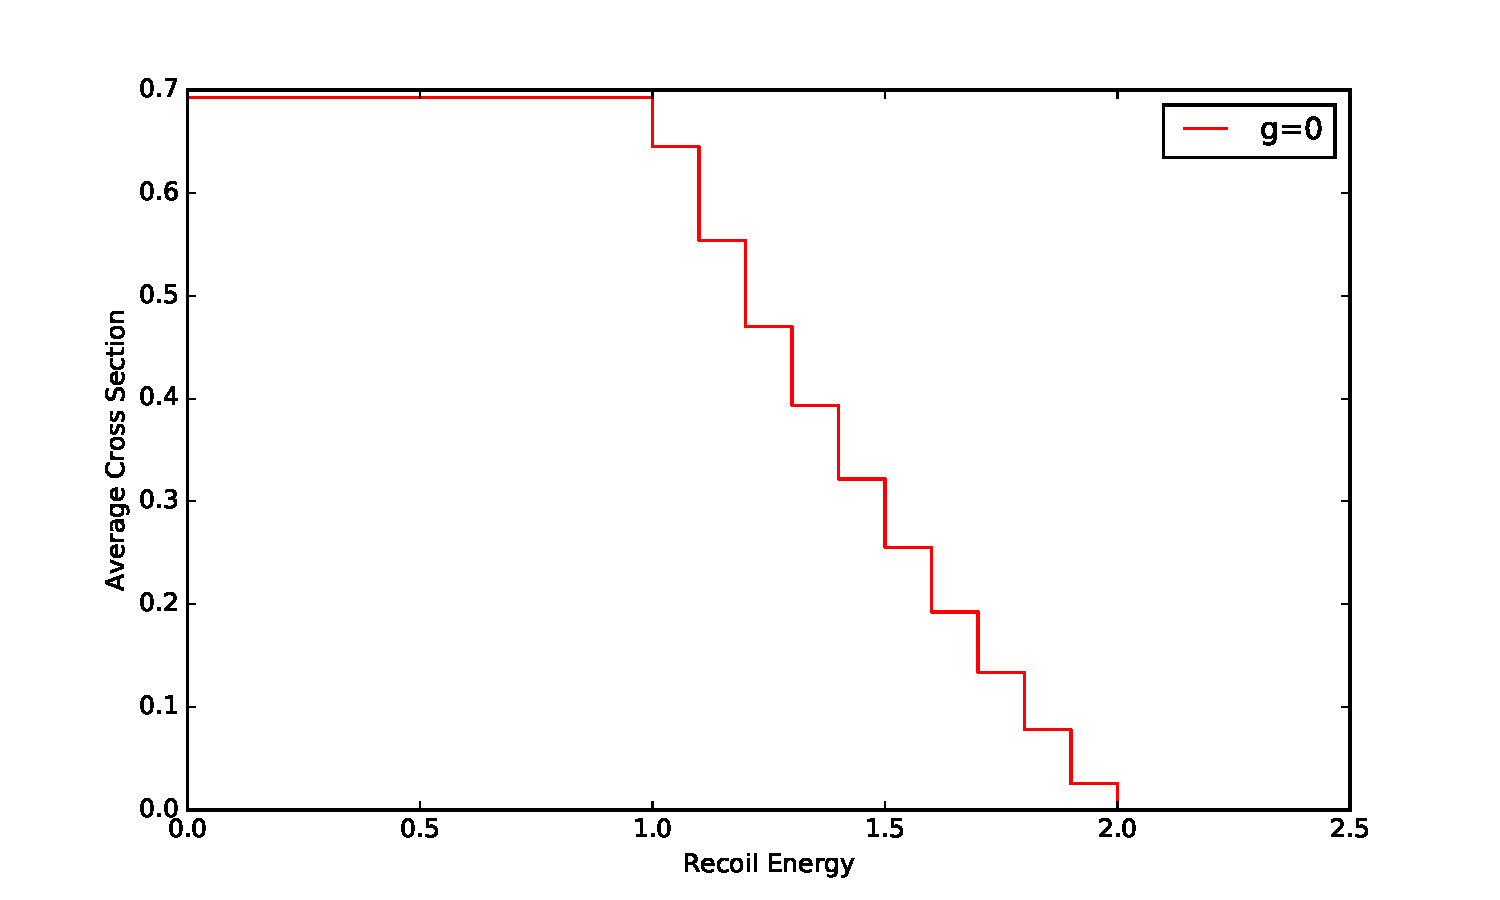
\includegraphics[width=1\linewidth]{erxs_analytical.pdf}
	\caption{Average recoil cross section of $^1$H given constant scattering cross section and spectrum, $ 1 < E < 2$.}
	\label{fig:analytical}
\end{figure}


%**********************************************************************************************************************************************************************************************%
\section{Verification of Elastic Scattering Cross Sections}
The first test uses a constant spectrum $\xi(E)=1$, constant recoil cross section $\sigma_{r,n}(E)=1$, hydrogen with $A=1$ as recoil nucleus. We focus on a neutron energy bounded by $E=[0,1]$ eV. The recoil energy groups have a width of $0.1$ eV and are uniformly distributed from $0$ to $2$ eV; $L$ is set to $0$. The expectation is that the average recoil cross section increases linearly between $1<T<2$ and remains constant between $0<T<1$.  Figure \ref{fig:analytical} shows the result obtained with the cross section preparation object behaves as expected. 
\begin{figure}[t!]
	\centering
	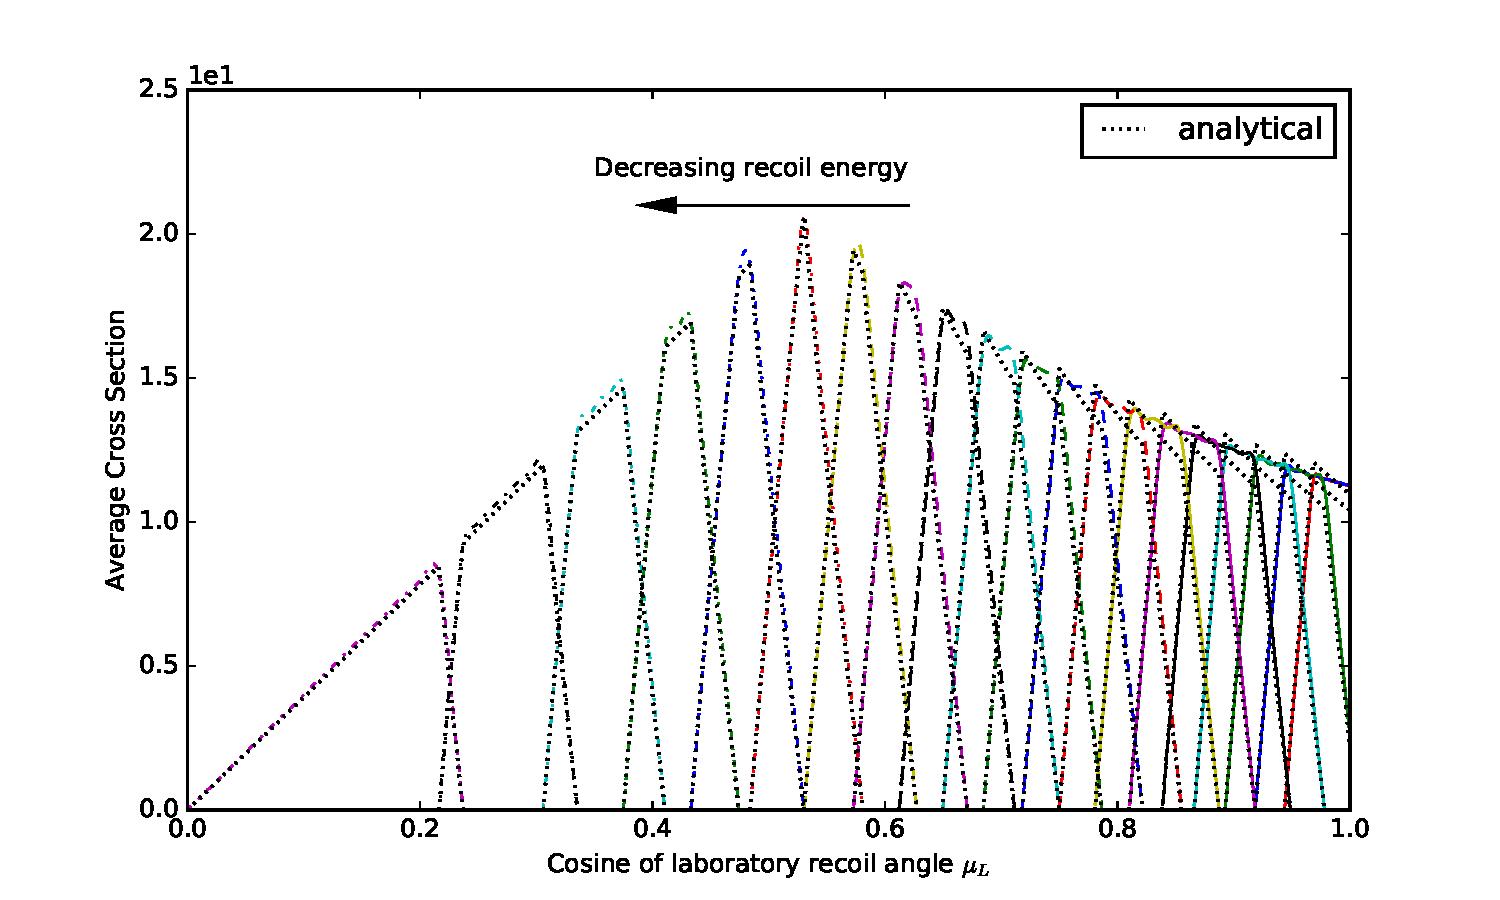
\includegraphics[width=1\linewidth]{erxs_analytical_mu.pdf}
	\caption{Value of the transfer cross section from neutron energy group $g=0$ to various recoil energy groups indexed by $t$.}
	\label{fig:analytical_vs_angle}
\end{figure}


The second test is to assert correctness of the computed angular distribution in the LAB frame. To this end, we compare results from the implemented algorithm with 
analytical results derived in section~\ref{sec:analytical_muL}. To reduce impact of wide energy bins, we use $1<E< 1.2$ and $\frac{j-1}{20}< T < \frac{j}{20}$ for $j=1,...,20$.
We select $A=2$ corresponding to $\gamma = 8/9$.

In Fig.~\ref{fig:analytical_vs_angle}, the value of the transfer cross section is plotted vs. the LAB scattering cosine $\mu_l$. The black dotted lines are the analytical reference for $j=1,..,20$ while the colorized lines are the results from the computation for $L=20$. 
The index $j$ of the curves increases from left to right as larger $j$ correspond to smaller energy transfer; in turn smaller energy transfer to the recoil corresponds to smaller LAB scattering cosines as shown in Eq.~\ref{eq:min_max_mu}. This behavior is reproduced in Fig.~\ref{fig:analytical_vs_angle}. The analytical results are in good agreement with the computed distributions. It should be noted that the angular distributions $p_{\mu_L}$ are not continously differentiable leading to relatively slow convergence of the numerical results to the analytical solution with increasing $L$.

%\section*{References}
\clearpage
\section*{References}
\bibliography{bibdata}

\end{document}